% Created 2022-10-05 Wed 21:13
% Intended LaTeX compiler: pdflatex
\documentclass[11pt]{article}
\usepackage[utf8]{inputenc}
\usepackage[T1]{fontenc}
\usepackage{graphicx}
\usepackage{longtable}
\usepackage{wrapfig}
\usepackage{rotating}
\usepackage[normalem]{ulem}
\usepackage{amsmath}
\usepackage{amssymb}
\usepackage{capt-of}
\usepackage{hyperref}
\author{Rafał Grot}
\date{\today}
\title{Matematyka 1 cos}
\hypersetup{
 pdfauthor={Rafał Grot},
 pdftitle={Matematyka 1 cos},
 pdfkeywords={},
 pdfsubject={},
 pdfcreator={Emacs 28.2 (Org mode 9.6)}, 
 pdflang={English}}
\begin{document}

\maketitle
\tableofcontents


\section{liczby zespolone}
\label{sec:org4048eae}
\begin{itemize}
\item \(\mathbb{Z}\) - zbiór liczb całkowitych
\item \(\mathbb{R}\) - zboór liczb rzeczywistych
\item \(\mathbb{C}\) - zbiór liczb zespolonych
\end{itemize}
$$\mathbb{Z} \subset \mathbb{R} \subset \mathbb{C}$$
\subsection{postać algerbraiczna liczby zespolonej}
\label{sec:org0aa5d27}
$$z=a+bi$$

Zapis zgodny z \url{https://en.wikipedia.org/wiki/Complex\_number} (prznynajmniej w części)
\begin{itemize}
\item \(\Re(z) = a\) - część rzeczywista liczby zespolonej.
\item \(\Im(z) = b\) - częśc urojona liczby zespolonej.
\item \(i\) - jednostka urojona \(i^2=-1\)
\end{itemize}
\subsubsection{sprzężenie liczby zespolonej}
\label{sec:org43b75b4}
$$z=a+bi$$
$$\overline{z}=a-bi$$
$$w=f-gi$$
$$\overline{w}=f+gi$$
\subsection{postać trygonometryczna liczby zespolonej}
\label{sec:org2180eab}
$$z=(z)(\cos\varphi*\sin\varphi)$$
\subsection{postać wykładnicza liczby zespolonej}
\label{sec:org9f29046}
$$z=(z)*e^{i\varphi}$$
\subsection{modół liczby zespolonej}
\label{sec:org8f11203}
$$$$
\begin{center}
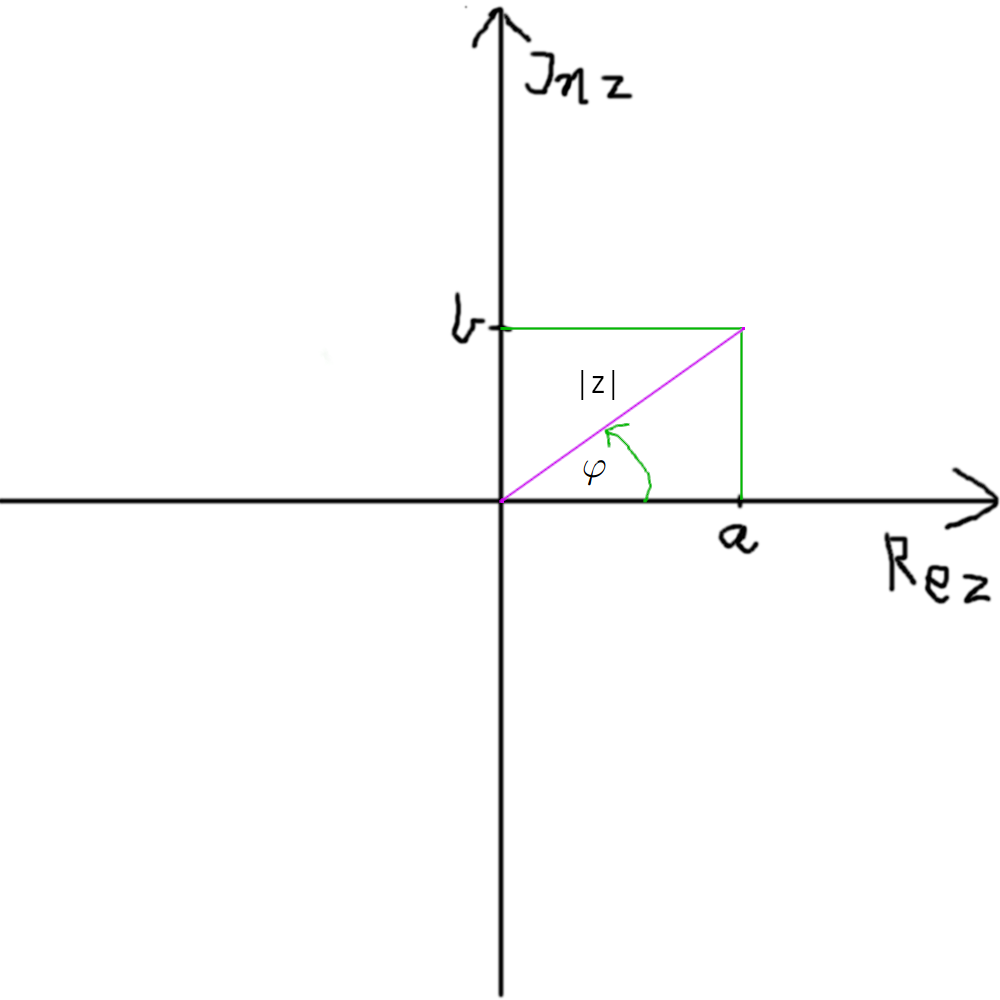
\includegraphics[width=.9\linewidth]{./figure01.png}
\end{center}

\(|z|=\sqrt{a^2+b^2}\)

\(\varphi\) - argument
\subsection{Potęgowanie liczby zespolonej}
\label{sec:orga23339d}
$$z=a+bi \to z=|z|(\cos \varphi + i \sin \varphi)^n \to |z|^n(\cos n \varphi + i \sin n \varphi)$$
\end{document}
